\documentclass[11pt]{article}
\usepackage[T1,T2A]{fontenc}
\usepackage[utf8]{inputenc}
\usepackage[english,russian]{babel}
\usepackage{graphicx}
\usepackage{amsmath}
\graphicspath {{img/}}

\title{\textbf{Лабораторная работа №4\\<<Исследование устройств частотного преобразования сигналов в системах передачи информации>>}}
\author{Перепелица А.А., ККСО-01-19}
\date{Москва, 2022 г.}
\addtolength{\topmargin}{-3cm}
\addtolength{\textheight}{3cm}
\begin{document}
\maketitle
\thispagestyle{empty}
\textbf{Цель работы:} ознакомление с устройством, работой частотных 
модуляторов и демодуляторов сигналов и приобретение практических навыков 
моделирования этих устройств. 

\section{Схема №1: исследование АМ сигналов}
\subsection{Перечень элементов, использованных в схемах, с
их краткими характеристиками}
\begin{itemize}
    \item[-] Источник переменного тока (3.54 В, 200 Гц, $90^\circ$)
    \item[-] Четырехканальный осциллограф
    \item[-] Источник напряжения частотной модуляции (5 В, 100/8 кГц) 2 шт.
    \item[-] Анализатор спектра 
    \item[-] Ключ
\end{itemize}


\subsection{Копии окон схемных файлов с позиционными обозначениями}
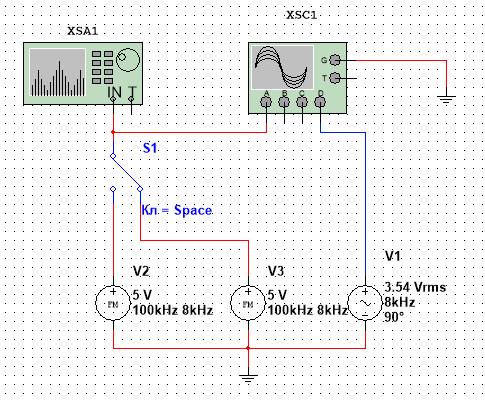
\includegraphics[width=1\linewidth]{img/scheme1.png}
\begin{center}
    Рис.1 Схема исследования ЧМ сигналов
\end{center}

\subsection{Результаты расчетов и измерений приборами}
\begin{center}
    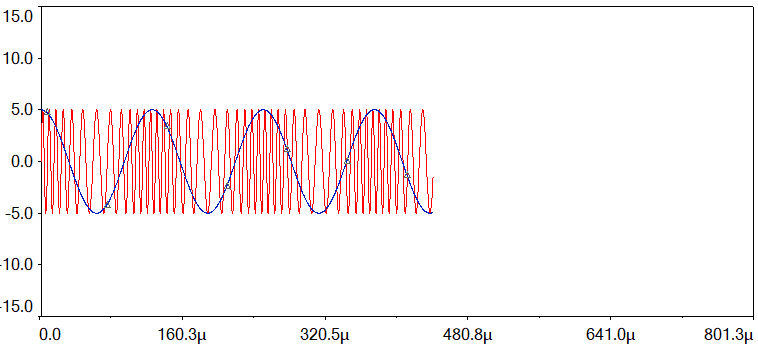
\includegraphics[width=1\linewidth]{img/osc1.png}
        Рис.2 Показания осциллографа при первом положении ключа.
\end{center}

\begin{center}
    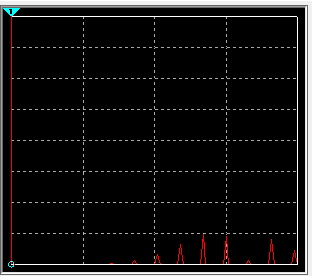
\includegraphics[width=1\linewidth]{img/chast1.png}
        Рис.3 Показания анализатора спектра при первом положении ключа.
\end{center}


\newpage
\section{Схема №2: исследование модели частотной манипуляции}
\subsection{Перечень элементов, использованных в схемах, с
их краткими характеристиками}
\begin{itemize}
    \item[-] Источник переменного тока (3.54 В, 200 Гц, $90^\circ$)
    \item[-] Четырехканальный осциллограф
    \item[-] Источник напряжения частотной модуляции (5 В, 100/8 кГц) 2 шт.
    \item[-] Анализатор спектра 
    \item[-] Ключ
\end{itemize}

\subsection{Копии окон схемных файлов с позиционными обозначениями}
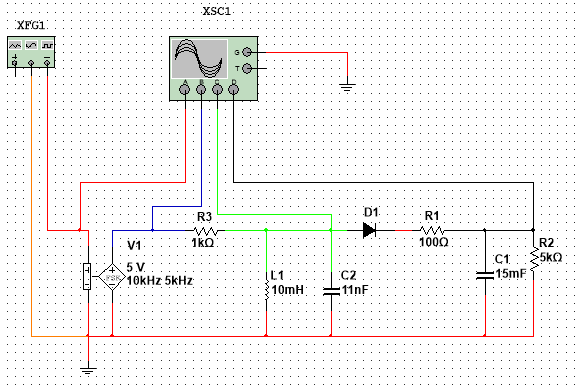
\includegraphics[width=1\linewidth]{img/scheme2.png}
\begin{center}
    Рис.4 Схема частотного модулятора и демодулятора
\end{center}

\subsection{Результаты расчетов и измерений приборами}
\begin{center}
    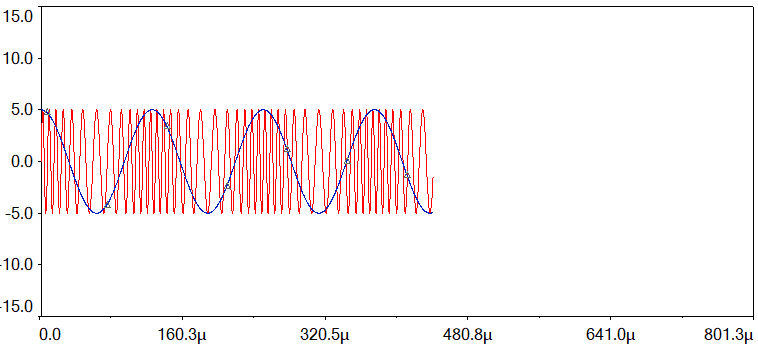
\includegraphics[width=1\linewidth]{img/osc1.png}
        Рис.5 Показания осциллографа при первом положении ключа.
\end{center}


\newpage
\section{Схема №3: Исследование модели системы передачи информации с частотной манипуляцией}
\subsection{Перечень элементов, использованных в схемах, с
их краткими характеристиками}
\begin{itemize}
    \item[-] Источник переменного тока (3.54 В, 200 Гц, $90^\circ$)
    \item[-] Четырехканальный осциллограф
    \item[-] Источник напряжения частотной модуляции (5 В, 100/8 кГц) 2 шт.
    \item[-] Анализатор спектра 
    \item[-] Ключ
\end{itemize}


\subsection{Копии окон схемных файлов с позиционными обозначениями}
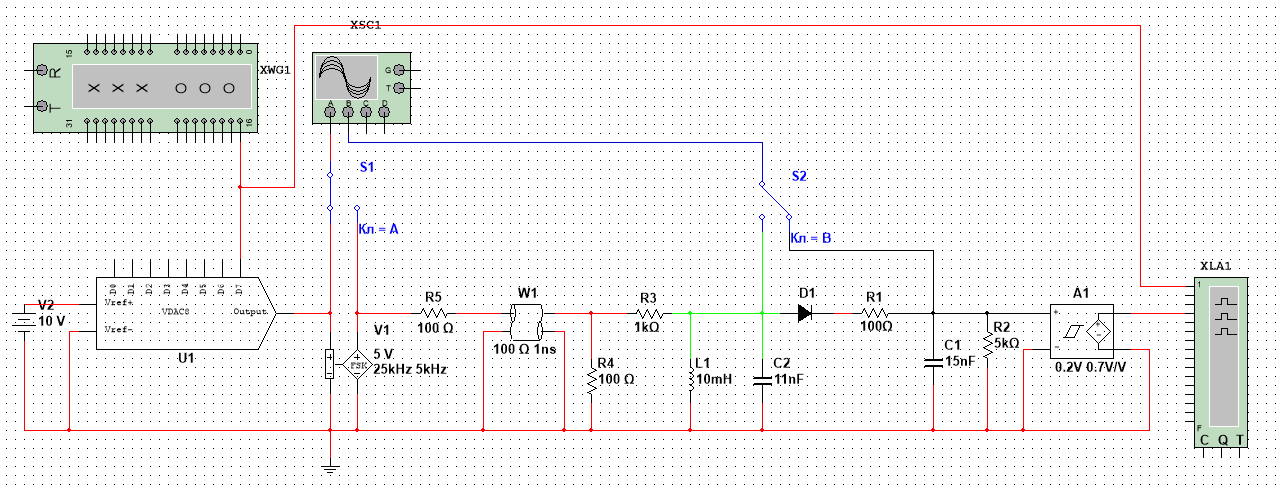
\includegraphics[width=1\linewidth]{img/scheme3.png}
\begin{center}
    Рис.7 Схема модели системы передачи информации с частотной манипуляцией
\end{center}

\subsection{Результаты расчетов и измерений приборами}
\begin{center}
    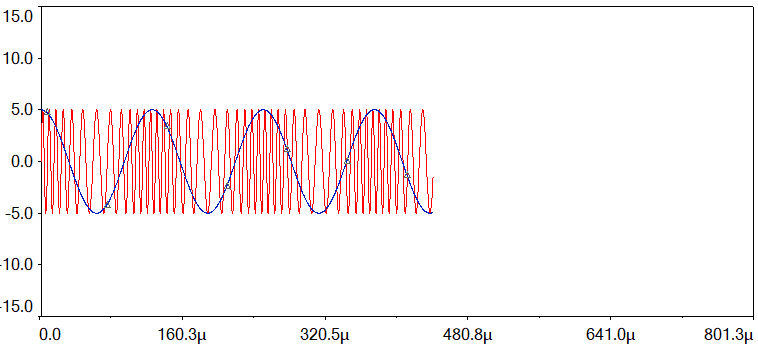
\includegraphics[width=1\linewidth]{img/osc1.png}
        Рис.8 Показания осциллографа при первом положении ключа.
\end{center}


\textbf{Вывод:} в ходе выполнения лабораторной работы мы изучили принцип передачи двоичных данных по сети связи, а также принципы работы и построения частотного модулятора и демодулятора.



\end{document}